% !TEX root = ../Bachelorthesis.tex
%
%************************************************
% Einführung
%************************************************
\chapter{Einführung}
\label{sec:Einfuehrung}

Springer Nature ist ein weltweit führender Verlag für Forschungs-, Bildungs- und Fachliteratur mit einer breiten Palette an angesehenen und bekannten Medienmarken und zudem der weltweit größte Verlag für Wissenschaftsbücher. Für das Unternehmen Springer Nature ist es darum wichtig, auf seinen Web-Applikationen eine Suche anbieten zu können, die Suchintentionen erkennt und möglichst schnell zum gesuchten Content leitet. Die Suche wird vor allem als Hilfsmittel zur Navigation und zum Finden von Literatur und Dienstleistungen genutzt. Durch die vielen von Springer Nature publizierten Zeitschriften und Querverweise in Artikeln, wird sie aber auch oft zur Suche nach Issues\footnote{Nummer der Zeitschriftenausgabe, in der sich der Artikel befindet.} und Artikeln verwendet sowie als Hilfestellung um Diagnosen zu Krankheitsbilder stellen zu können.
\\
\\
Springer Nature sammelt viele User-Tracking-Daten und dadurch viel Wissen über das Verhalten der User\footnote{Als User werden die Nutzer der Springermedizin-Suche bezeichnet} bei der Nutzung ihrer Suche, lässt dieses Wissen jedoch bisher noch nicht in ihre Suche einfließen. In dieser Arbeit wollen wir untersuchen, ob mithilfe dieses Wissens, die Suche optimiert werden kann.

\section{Aufbau der Suche bei Springer Nature}
\label{sec:Einfuehrung:AufbauSucheBeiSpringerNature}

\subsubsection{White Label Applikation mit Solr-Suche}
\label{sec:Einfuehrung:AufbauSucheBeiSpringerNature:WhiteLabelApplikationSolr-Suche}

Damit die verschiedenen Verlage und Zeitschriften der Verlagsgruppe Springer Nature ihre Produkte und Dienstleistungen online anbieten können nutzt Springer Nature eine eigens entwickelte White Label Applikation\footnote{Eine White Label Applikation ist eine wiederverwendbare und agil erweiterbare Applikation}. Die White Label Applikation verwendet \textit{Apache Solr}\footnote{http://lucene.apache.org/solr} (im Folgenden "Solr" genannt) als Suchplattform. Die Solr dient hierbei als eine der Schnittstellen zwischen dem Content-Pool von Springer Nature und der White Label Applikation. Bei den vom Content-Pool gelieferten Inhalten, handelt es sich um von Springer Nature Verlag publizierte Zeitschriften, Artikel, Bücher und redaktionelle Inhalte.

\subsubsection{User-Tracking mit Webtrekk}
\label{sec:Einfuehrung:AufbauSucheBeiSpringerNature:Webtrekk}

Um das Verhalten der User auf ihren Web-Applikationen zu tracken verwendet Springer Nature das Analysetool Webtrekk\footnote{https://www.webtrekk.com}. Die daraus resultierenden Berichte bieten unter anderem die Möglichkeit, \textit{Suchquery-Logs}\footnote{Protokoll über alle ausgeführten Suchanfragen auf der Applikation} und \textit{Click-Trough-Rates} (CTR)\footnote{Kennzahl um die Anzahl der Klicks auf Links im Verhältnis zu den gesamten Impressionen darzustellen} der User auszuwerten.

\pagebreak

\subsubsection{Architektur}
\label{sec:Einfuehrung:AufbauSucheBeiSpringerNature:Architektur}

In Abb. \ref{fig:SucheSpringerNature} ist die Suche nochmals grafisch aufbereitet:

\begin{figure}[H]
\centering
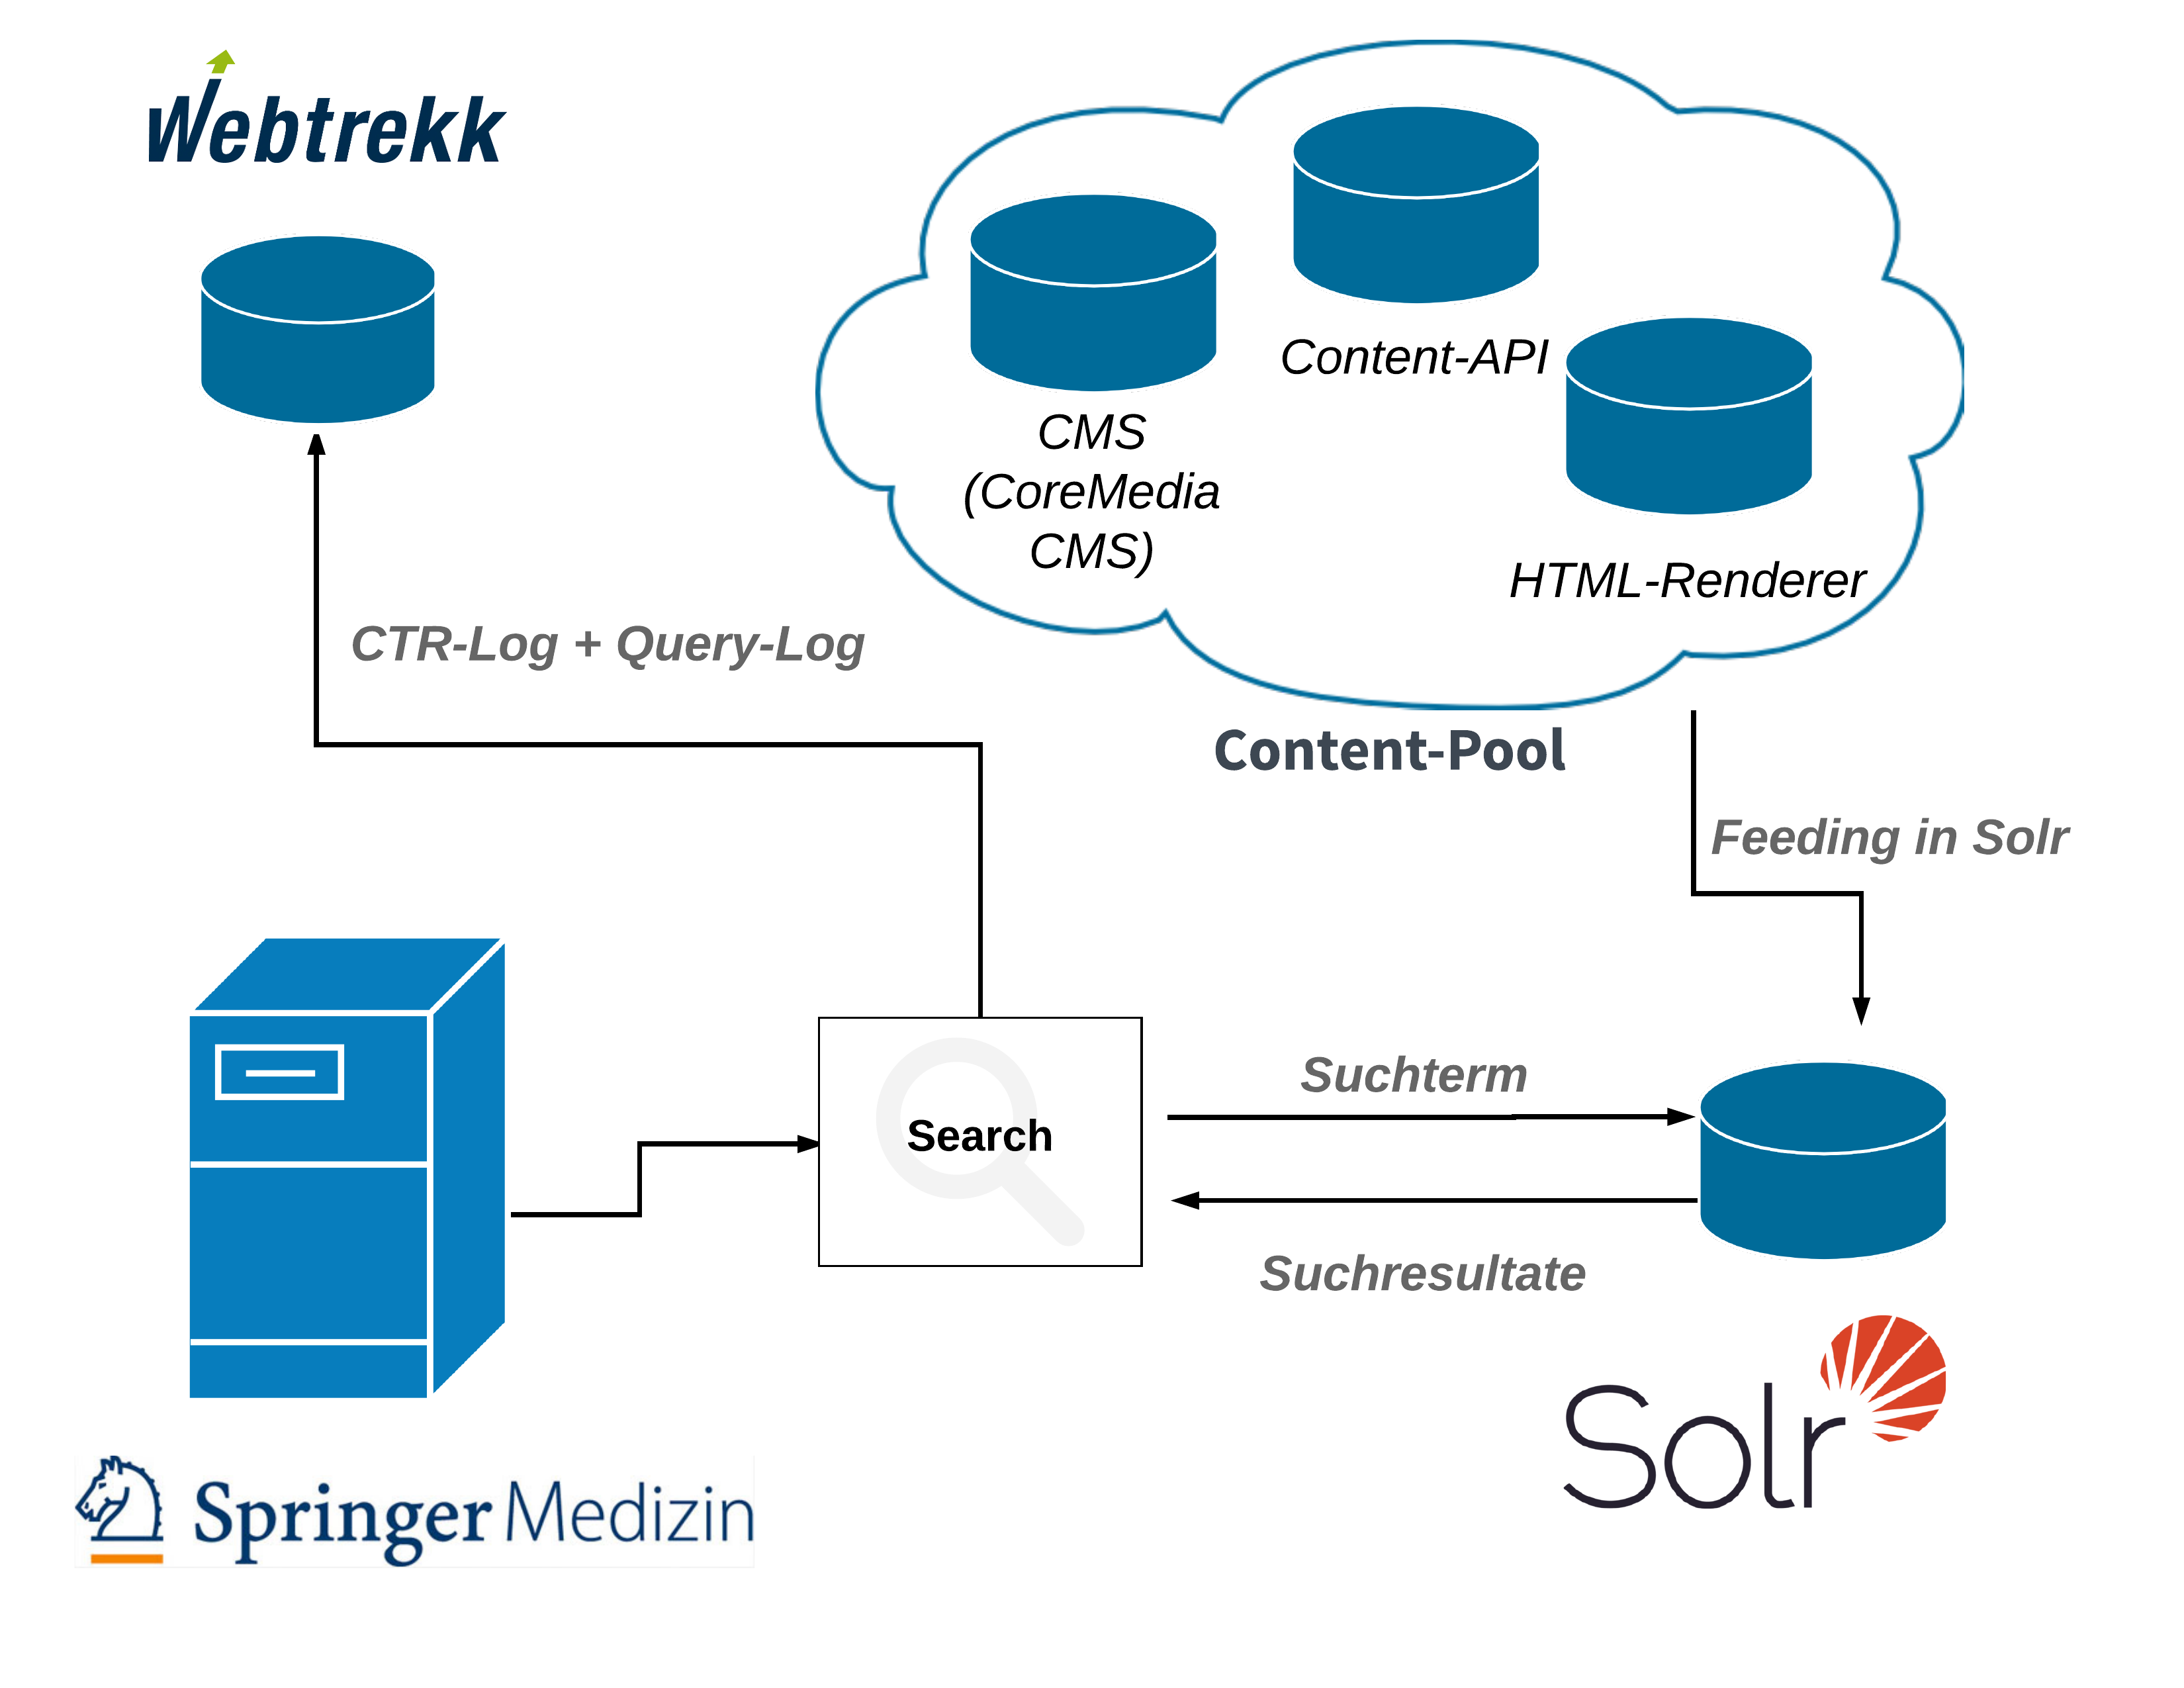
\includegraphics[width=0.5\linewidth]{gfx/AufbauSucheSpringerNature}
\caption[Aufbau der Suche bei Springer Nature]{Aufbau der Suche bei Springer Nature}
\label{fig:SucheSpringerNature}
\end{figure}

\section{Problemstellung: Keine Userrelevanz in der Suche}
\label{sec:Einfuehrung:Problemstellung}

\subsubsection{Userrelevante Dokumente werden nicht gefunden}
\label{sec:Einfuehrung:Problemstellung:Userrelevanz}

Die User von Springermedizin suchen oft mit einschlägig, fundierten Fachbegriffen nach den neuesten und relevantesten Zeitschriften, Bücher oder Publikationen. Die zeitlich aktuellsten Suchtreffer zu finden ist für Springermedizin kein Problem. Die für den User \textit{relevantesten} jedoch schon.

\subsubsection{Der Springer Nature Stakeholder: Springermedizin setzt auf Webtrekk}
\label{sec:Einfuehrung:Problemstellung:Springermedizin}

Zu den Stakeholder\footnote{Bezeichnet Springer Nature interne Kunden, die ein Interesse am Ergebnis der White Label Applikation haben} der in Kapitel \ref{sec:Einfuehrung:AufbauSucheBeiSpringerNature:WhiteLabelApplikationSolr-Suche} angesprochenen White Label Applikation gehört \textit{Springermedizin}\footnote{https://www.springermedizin.de/}. Springermedizin ist ein Fortbildungs- und Informationsportal für Ärzte. Mithilfe von Webanalysten und Webtrekk versucht Springermedizin das Marketing seines Webauftrittes zu verbessern und ist sehr interessiert an neuen Ansätzen, um die gesammelten Tracking-Daten besser einzusetzen. In dieser Arbeit wird darum der Fokus auf die Verwendung von Tracking-Daten in der Suche von Springermedizin gesetzt. 
 

\subsubsection{Der fast gläserne User}
\label{sec:Einfuehrung:Problemstellung:Glaeserne-User}

Springermedizin sammelt Tracking-Daten über jegliche Aktivitäten auf deren Applikationen und investiert Zeit und Geld in die Individualisierung\footnote{Mit Individualisierung wird die Speicherung eigener Parameter bezeichnet} der Analysedaten auf Webtrekk. Mittlerweile sind knapp 30 Custom-Parameter\footnote{Individuell erzeugte Parameter für Berichte und Analysen} auf Webtrekk angelegt um genau die Daten zu tracken, die zur Analyse des Verhaltens der User auf ihrer Applikationen relevant sind. Dadurch entsteht ein fast \glqq gläsernen User\grqq{}. Dieses Wissen könnte zum Vorteil des Users eingesetzt werden, indem es in der Suche verwendet wird.

\section{Ziel der Arbeit}
\label{sec:Einfuehrung:ZielArbeit}

\subsection{Suchoptimierung durch Click-Trough-Daten}
\label{sec:Einfuehrung:ZielArbeit:Suchoptimierung}

In dieser Arbeit werden wir untersuchen, ob mithilfe der von Springermedizin gesammelten Click-Trough-Daten dessen Suche verbessert werden kann. Im Idealfall widerspiegeln die gesammelten Click-Trough-Daten der Suchresultate die Userrelevanz der einzelnen Dokumente\footnote{Als Dokumente werden die einzelnen Suchresultate bezeichnet}.

\subsubsection{Annahmen}
\label{sec:Einfuehrung:ZielArbeit:Suchoptimierung:Annahmen}

Wir gehen dabei von folgenden Annahmen aus. Relevante Dokumente sind wichtiger als nicht relevante Dokumente. Eine Suchergebnis ist dann gut, wenn die relevanten Ergebnisse in der verwendeten Hierarchie vor den nicht relevanten Ergebnisse auftauchen. 

\subsection{Abbildung auf das Springermedizin-Umfeld}
\label{sec:Einfuehrung:ZielArbeit:AbbildungSpringermedizinUmfeld}

\subsubsection{Potential von Userrelevanzen in der Suchoptimierung analysieren}
\label{sec:Einfuehrung:ZielArbeit:Potential}

Die Analyse von User-Tracking-Daten bietet viel Potential bezogen auf Userrelevanzen. Sind anhand des hier umgesetzten Lösungsansatzes Verbesserungen in der Qualität der Suche zu verzeichnen, möchte Springermedizin in Zukunft vermehrt User-Tracking-Daten in die Suche einfließen lassen. Diese Arbeit könnte dann als Fundament für weitere Lösungsansätze dienen.

\subsubsection{Bekanntes und wirkungsvolles Information Retrieval Verfahren}
\label{sec:Einfuehrung:ZielArbeit:AbbildungSpringermedizinUmfeld:InformationRetrievalVerfahren}

Suchoptimierung mittels Userrelevanz ist ein bekanntes und nicht triviales, aber relativ wirkungsvolles Information Retrieval Verfahren (siehe \cite{IWUSBI}). Seit Mitte der 2000er Jahre wird mithilfe dieses Verfahrens versucht, Suchmaschinen zu verbessern. Aus dieser Zeit stammen auch die ersten Ansätze um mithilfe von Click-Trough-Daten die Userrelevanz der Suchergebnisse zu berechnen (siehe \cite{Joachims}).

\subsubsection{Lösungsansatz basierend auf Click-Trough-Daten aus Webtrekk}
\label{sec:Einfuehrung:ZielArbeit:AbbildungSpringermedizinUmfeld:Loesungsansatz}

Springermedizin führt ein eigenes Tracking der User durch und verwendet auf Webtrekk selbst definierte Tracking-Parameter. Dadurch hängt die Wahl des in dieser Arbeit zu untersuchenden Lösungsansatzes und dessen Umsetzung stark von den durch Webtrekk gegeben Analyse-Daten ab.

\subsubsection{Anwendung auf Springermedizin-Umfeld}
\label{sec:Einfuehrung:ZielArbeit:AbbildungSpringermedizinUmfeld:Adaptierung}

Bei der Verwendung von Userrelevanzen in der Suche handelt es sich um ein bekanntes und gut erforschtes Problem. Wir werden in dieser Arbeit versuchen, einen bestehenden Lösungsansatz (Die Wahl des Lösungsansatz folgt in Kapitel \ref{sec:Einfuehrung:Methodik:SucheEinbinden:PBM}) auf das Springermedizin-Umfeld abzubilden. Die Herausforderung wird hierbei die Adaptierung des Lösungsansatzes auf das Springermedizin-Umfeld sein.

\subsubsection{Was wird in dieser Arbeit nicht behandelt?}
\label{sec:Einfuehrung:ZielArbeit:AbbildungSpringermedizinUmfeld:NichtBehandeln}

Durch den vorgegebenen Zeitraum für die Erstellung dieser Bachelorarbeit bedingt, werden wir den Lösungsansatz so wählen, dass er mit den Gegebenheiten bei Springermedizin sinnvoll und in diesem Zeitrahmen realistisch implementiert werden kann. Wir werden daher in dieser Arbeit keine Gegenüberstellung mit anderen Lösungsansätzen machen. 
\\
\\
Bei der Umsetzung des Lösungsansatzes konzentrieren wir uns auf die Implementation des Algorithmus zur Berechnung der Userrelevanz. Die semantische Aufschlüsselung von Suchtermen ist nicht Kern dieser Arbeit. Die semantische Aufschlüsselung des Suchterms\footnote{Als Suchterm wird eine Suchanfragen bezeichnet} zur Analyse der Webtrekk-Daten enthält darum keine Gewichtungen der Relationen zwischen Webtrekk-Daten und Suchterm. Alle Relationen werden gleich gewichtet. 

\section{Methodik}
\label{sec:Einfuehrung:Methodik}

Wie in Kapitel \ref{sec:Einfuehrung:ZielArbeit:Suchoptimierung} angesprochen, wollen wir das Klickverhalten der User in der Suche analysieren um die Suchergebnisse zu verbessern.

\subsection{Analyse der Click-Trough Daten}
\label{sec:Einfuehrung:Methodik:Click-Trough-Daten}

\subsubsection{Userrelevante Dokumente durch Click-Trough-Rates identifizieren}
\label{sec:Einfuehrung:Methodik:Click-Trough-Daten:UserrelevanteDokumente}

Eine Möglichkeit, die Userrelevanz eines Suchergebnisses zu bestimmen, ist die Verwendung der Click-Trough-Daten zur Berechnung der Userrelevanz. Anhand der Click-Trough-Rates der Suchergebnisse, können wir die für die Nutzer der Suche relevanten Dokumente identifizieren.

Dazu analysieren wir, welche Dokumente im Suchergebnis zu welchen Suchtermen angeklickt worden sind. Wir gehen dabei davon aus, dass jedes Dokument, welches zu einer Suchanfrage angeklickt wurde, eine gewisse Relevanz für diese hat.

\subsubsection{Click-Trough-Daten kommen aus Webtrekk-Analysen}
\label{sec:Einfuehrung:Methodik:Click-Trough-Daten:Click-Trough-DatenWebtrekk-Analysen}

Als Wissensbasis zur Berechnung der Click-Trough-Daten dienen die Webtrekk-Analysen von Springermedizin. Wir können anhand dieser Analysen feststellen, welches Dokument zu welchem Suchterm angeklickt wurde. Wir wissen dadurch, wie oft es angeklickt wurde und auf welcher Position\footnote{Mit Position wird der dargestellte Rang des Dokumentes im Suchresultat bezeichnet} im Suchresultat sich das Dokument dabei befunden hat. 

\subsubsection{Suchterm semantisch aufschlüsseln mittels Segmentierung}
\label{sec:Einfuehrung:Methodik:Click-Trough-Daten:SuchtermSegmentierung}

Ein Suchterm kann aus mehr als einem Wort bestehen. Wir müssen darum davon ausgehen, dass möglicherweise jedes Wort des Suchterms in unterschiedlichen Suchanfragen verwendet wird. Außerdem kann auch nach Synonymen eines Wortes gesucht werden. Der Suchterm muss darum semantisch aufgeschlüsselt werden, um alle relevanten Click-Trough-Daten berechnen zu können. Die Click-Trough-Daten sind dann relevant, wenn mindestens ein Wort des aufgeschlüsselten Suchterms in Relation zu diesen Daten steht. Von einer Gewichtung der Relation wird abgesehen.
\\
\\
Die Auftrennung des Suchterms in die einzelne Worte können wir mithilfe einer Segmentierung\footnote{Bezeichnet die Aufteilung in Abschnitte, in diesem Fall in einzelne Worte} durchführen. Hier könnten wir uns überlegen, zusätzlich mit Stoppwörtern\footnote{Stoppwörter sind Wörter, die sehr häufig auftreten und für gewöhnlich keine Relevanz für den Dokumentinhalt besitzen} nicht relevante Wörter aus dem Suchterm zu entfernen. Dieses Verfahren macht aber im Springermedizin-Kontext keinen sein. Wie in Kapitel \ref{sec:Einfuehrung:Problemstellung:Userrelevanz} angesprochen, suchen die User der Springermedizin-Applikation oft mit einschlägig, fundierten Fachbegriffen. Wir gehen darum davon aus, dass alle Wörter des verwendeten Suchterms für das Suchergebnis relevant sind. Diese Erkenntnis basiert auf Aussagen der Redakteure von Springermedizin und Webtrekk-Analysen der meist gesuchtesten Suchtermen der letzten Monate. Auch sind Stoppwörter veraltet und werden in modernen Information Retrieval Verfahren nicht mehr eingesetzt. Wir verzichten darum auf den Einstatz von Stoppwörtern.

\subsubsection{Suchterm semantisch erweitern mittels Thesaurus}
\label{sec:Einfuehrung:Methodik:Click-Trough-Daten:SuchtermThesaurus}

Für die semantische Erweiterung eines Suchwortes wird ein Thesaurus\footnote{Als Thesaurus wird ein strukturiertes Verzeichnis von Begriffen, welche allesamt in irgendeiner Beziehung stehen bezeichnet} benötigt. Die Erweiterung umfasst zum Suchterm gleichbedeutende Begriffe (Synonyme), sehr ähnliche Begriffe (Narrow Terms), ähnliche Begriffe im weiteren Sinne (Broader Terms) und verwandte Begriffe (Related Terms).
\\
\\
Springer Nature besitzt einen Webservice mit welchem auf den Thesaurus \textit{Unified Medical Language System}\footnote{https://www.nlm.nih.gov/research/umls/} (UMLS) zugegriffen werden kann. 

\subsubsection{Komplexe Auswertungen der Click-Trough-Daten nicht möglich}
\label{sec:Einfuehrung:Methodik:Click-Trough-Daten:Click-Trough-DatenAuswertungen}

Die Webtrekk-Analysen bieten uns jedoch nur beschränkte Informationen zum Klickverhalten der User. Wichtige Informationen wie die Verweildauer auf einem Dokument oder ob nach diesem Dokument ein weiteres Dokument zum gleichen Suchterm angeklickt worden ist, lassen diese Analysen nicht zu. Da diese Informationen für komplexe Auswertungen der Click-Trough-Daten nicht ausreichen, können wir in dieser Arbeit \textit{Feedback-Strategien} für die Click-Trough-Rate Auswertung, wie in \cite{Joachims} beschrieben, nicht verwenden. Stattdessen müssen wir davon ausgehen, dass jeder Klick auf ein Dokument relevant ist.

\subsubsection{Durch Webtrekk kein komplexer Lern-Algorithmus notwendig}
\label{sec:Einfuehrung:Methodik:Click-Trough-Daten:Lern-Algorithmus}

Der Vorteil bei der Verwendung von Webtrekk ist, dass der Algorithmus nicht stetig neues Wissen lernen und altes vergessen muss. Der Algorithmus kann direkt zur Laufzeit\footnote{Unter Laufzeit wird in diesem Fall der Zeitpunkt der direkte Abfrage während der Suchanfrage bezeichnet} Analysen gegen Webtrekk über eine frei definierbare Periode machen. Dadurch kann \textit{overfitting}\footnote{Überanpassung des Algorithmus durch zu viele (falsche oder veraltete) Daten} vermieden werden. Deshalb werden wir von komplexen Lern-Algorithmen wie in \cite{IWUSBI} vorgestellt, absehen.

\subsection{Userrelevanz in Suchprozess einbinden}
\label{sec:Einfuehrung:Methodik:SucheEinbinden}

Es gibt drei mögliche Eingriffspunkte während des Suchprozesses, um Userrelevanzen in der Springermedizin-Suche zu verwenden. Möglich wäre die Verwendung der Userrelevanzen in der Aufbereitung der Suchanfrage auf der Springermedizin-Applikation. Denkbar wäre auch, die Berechnung der Userrelevanzen in den Suchindex der Solr einzubauen. Die dritte Variante wäre die Verwendung der Userrelevanzen in der Aufbereitung der Suchresultate der Springermedizin-Applikation. Eine davon, wollen wir in dieser Arbeit untersuchen. 

\subsubsection{Ansatz: Suchindex-Erweiterung in der Solr-Suche}
\label{sec:Einfuehrung:Methodik:SucheEinbinden:SolrSuche}

Um die Userrelevanzen direkt in die Solr einzubeziehen gibt es zwei Varianten. Wir können das Schema des Suchindexes über die Schema API\footnote{https://cwiki.apache.org/confluence/display/solr/Schema+API} erweitern und alle Einträge neu indexieren, oder wir ergänzen den Index um ein externes Feld\footnote{https://lucene.apache.org/solr/5\_4\_1/solr-core/org/apache/solr/schema/ExternalFileField.html} (ExternalFileField).
\\
\\
Beide Lösungsansätze ergeben nur bei der Speicherung einer einfachen Click-Count Popularität\footnote{Kennzahl für alle Klicks auf ein Dokument unabhängig des Suchterms} Sinn. Diese genügen allerdings den hier gegebenen Anforderungen nicht, da die Click-Trough-Rate abhängig vom Suchterm ist. Der erste Lösungsansatz ist zudem besonders heikel, weil bei jeder Änderung des Click-Count-Wertes, das Dokument in der Solr neu indexiert werden.

\subsubsection{Ansatz: Aufbereitung der Suchanfrage}
\label{sec:Einfuehrung:Methodik:SucheEinbinden:Suchanfrage}

Die Solr-Suche bietet eine Boost-Funktion namens \textit{DisMax Query Parser}\footnote{https://cwiki.apache.org/confluence/display/solr/The+DisMax+Query+Parser}.  Mit dieser können basierend auf Feldwerten, einzelne Dokumente besser im Suchergebnis positioniert werden. Die Boost-Funktion müssten wir in den Aufbau der Suchanfrage für die Suche auf der Springermedizin-Applikation einbauen. Dieser Ansatz beinhaltet einige Gefahren die wir beachten müssen.
\\
\\
Dazu zählen beispielsweise die Abhängigkeiten von anderen Boost-Faktoren\footnote{Die Solr besitzt eine Boosting-Funktion, mit welcher bestimmte Wertübereinstimmungen in der Suche höher gewichtet werden können}. Alle Boost-Faktoren hängen voneinander ab und müssten bei jeder Ergänzung um neue Faktoren normalisiert werden, um kein \glqq über-Boosting\grqq{}\footnote{Bezeichnet die über-priorisierte Bewertung einzelner Faktoren} einzelner Faktoren zu riskieren. Zudem besteht die Gefahr des \glqq blinden Boosting\grqq{} von Dokumenten. Die Solr-Relevanzberechnung ist komplex und der Einfluss des \glqq Boosting\grqq{} in die Solr-Relevanzberechnung schwer erkennbar. Auch hat Springermedizin bereits sehr schlechte Erfahrungen mit \glqq Boosting\grqq{} gemacht und bevorzugt einen Lösungsansatz ohne \glqq Boosting\grqq{}.

\subsubsection{Ansatz: Aufbereitung der Suchresultate anhand eines Klick-Modell basierten Algorithmus}
\label{sec:Einfuehrung:Methodik:SucheEinbinden:Suchresultate}

Die dritte Möglichkeit ist bei der Aufbereitung der Suchresultate aus der Solr-Suche einen Klick-Modell (siehe \cite{pbm}) basierten Algorithmus zu verwenden. Dieser soll die Suchergebnisliste analysieren, die Userrelevanzen der Dokumente berechnen und die Liste neu sortieren. 
\\
\\
Diese Lösung können wir relativ einfach in die Springermedizin-Applikation integrieren, ohne die restliche Suchlogik\footnote{Dazu gehört die Aufbereitung der Suchanfrage für die Solr und die Suche auf der Solr} zu beeinflussen. Hierbei müssen wir jedoch beachten, dass die Solr durch die Pagination-Funktion\footnote{https://cwiki.apache.org/confluence/display/solr/Pagination+of+Results} nur die Top-N-Ergebnisse (bei Springermedizin sind es 20 Ergebnisse) zurückgibt. Diese Logik liegt in der Springermedizin-Applikation im Aufbau der Suchanfrage. Daher können wir diese selber steuern und uns statt 20 beispielsweise die nächsten 100 Ergebnisse zurückgeben lassen. Am Ende filtern wir die ersten 20 Ergebnisse und stellen diese dar. Außerdem wissen wir bei diesem Lösungsansatz, in welcher Reihenfolge die Ergebnisse aus der Solr zurückgegeben werden. Wir kennen die Dokumente und deren Rang. Dadurch haben wir hilfreiches Zusatzwissen, welches wir in den Klick-Modell basierten Algorithmus einfließen lassen können.

\subsubsection{Entscheidung für den Ansatz der Aufbereitung der Suchresultate anhand eines Klick-Modell basierten Algorithmus}
\label{sec:Einfuehrung:Methodik:SucheEinbinden:Entscheidung}

Wägen wir die besprochenen Fakten ab, wirkt der Ansatz mit der Aufbereitung der Suchresultate durch einen Klick-Modell basierten Algorithmus am sinnvollsten. Wir wissen bei diesem Ansatz, welche Dokumente für die Userrelevanz-Berechnung überhaupt in Frage kommen. Zudem kennen wir alle Einfluss-Faktoren für den Algorithmus und wir sind unabhängig von der Suchlogik auf der Solr. Dadurch können wir Änderungen in unserer Logik schnell und einfach implementieren.

\subsubsection{Klick-Wahrscheinlichkeit mit Position-based Modell berechnen}
\label{sec:Einfuehrung:Methodik:SucheEinbinden:PBM}

Mithilfe der Click-Trough-Daten aus Webtrekk, können wir zwei wichtige Informationen zu jedem Suchterm ermitteln. Wir wissen welche Dokumente und welche Positionen im Suchresultat angeklickt worden sind. Zudem kennen wir die Reihenfolge der Dokumente im Suchresultat der Solr.
\\
\\
Ein Ansatz der genau auf diesen Informationen aufbaut, ist das \textit{Position-based Modell} (PBM)\cite{pbm}. Dieses berechnet die Wahrscheinlichkeit dafür, dass ein User ein Dokument wirklich genau analysiert, bevor er es anklickt. Es setzt sich aus zwei Wahrscheinlichkeiten zusammen. Die Wahrscheinlichkeit für einen Klick auf die Position im Suchresultat und die Wahrscheinlichkeit für einen Klick auf das Dokument. Diesen Ansatz werden wir in dieser Arbeit implementieren.

\subsubsection{Verhältnis zwischen den Klick-Wahrscheinlichkeiten abhängig der Position im Suchresultat definieren}
\label{sec:Einfuehrung:Methodik:SucheEinbinden:PBM}

Aus eigener Erfahrung wissen wir, dass die ersten Dokumente im Suchresultat immer zuerst gesehen werden. Die dahinter gelisteten Dokumente werden fortlaufend analysiert. Wir sollten darauf achten, dass je \textit{schlechter} der Rang des angeklickten Dokumentes im Suchresultat der Solr ist, desto \textit{höher} das Relevanzfeedback zu bewerten ist.

\subsubsection{Smoothing Faktor in Position-based Modell}
\label{sec:Einfuehrung:Methodik:SucheEinbinden:SmoothingPBM}

Wir wissen dass eine Wahrscheinlichkeit einen Wert zwischen 1 und 0 besitzt. Dadurch können Nullwerte entstehen. Das PBM multipliziert die Positions- und Dokument-Wahrscheinlichkeit miteinander, um die Klick-Wahrscheinlichkeit zu berechnen. Wir müssen aber davon ausgehen, dass es Dokumente geben kann, deren Rang nie angeklickt worden ist und umgekehrt. 
\\
\\
Multiplikationen mit Null ergeben immer einen Nullwert. An dieser Stelle führen wir einen \glqq Smoothing-Faktor\grqq{} ein. Der Smoothing-Faktor soll zwei Probleme lösen. Zum einen wollen wir einen Wahrscheinlichkeitswert trotz der Multiplikation mit Null beachten. Zum anderen wollen wir die im vorherigen Absatz beschriebene Gewichtung abhängig des Relevanzfeedbacks in den Algorithmus einbeziehen. Wir transformieren dazu das Produkt der beiden Wahrscheinlichkeiten in eine gewichtete Summe, dem sogenannten "Weighted Moving Average", dessen Gewichte sich zu Eins aufsummieren. Diese Gewichte sind die Smoothing-Faktoren, weshalb das Verfahren zählt zu den Smoothing-Algorithmen zählt.

\subsection{Effektive Userrelevanz}
\label{sec:Einfuehrung:Methodik:Userrelevanz}

\subsubsection{Die Klick-Wahrscheinlichkeit ist kein absoluter Wert für Userrelevanz}
\label{sec:Einfuehrung:Methodik:Userrelevanz:Relevanzfeedback}

Nun könnten wir die Klick-Wahrscheinlichkeit als absoluten Wert für die \textit{Userrelevanz} betrachten. Dies wäre jedoch falsch, wir müssen davon ausgehen, dass viele User der Qualität der Suchmaschine vertrauen. Diese betrachten die Top-Suchresultate als die relevanten Suchresultate. Denkbar wäre auch, dass sie unabsichtlich das falsche Dokument anklicken.

\subsubsection{Overfitting vermeiden}
\label{sec:Einfuehrung:Methodik:Userrelevanz:Overfitting}

Um dem entgegenzuwirken und ein \textit{overfitting} zu vermeiden, darf der Algorithmus nicht immer anschlagen. Wir müssen sicherstellen, dass vereinzelt zufällige Dokumente in den \glqq Top-Suchresultaten\grqq{} angezeigt werden. So können auch andere Dokumente in den Fokus des Users gerückt werden. Das System fährt sich dadurch nicht auf falschen Annotationen fest. 

\subsubsection{Zusätzliche Varianz durch Zufallsfaktor}
\label{sec:Einfuehrung:Methodik:Userrelevanz:Zufallsfaktor}

Mithilfe eines Zufallsfaktors kann eine solche Varianz in den Klick-Modell basierten Algorithmus gebracht werden. Wie bereits weiter oben erwähnt, werden viele Suchresultate nie und deren Rang selten bis gar nicht angeklickt. Sie haben darum keine Click-Trough-Daten. Deren Klick-Wahrscheinlichkeit ist entweder Null oder sehr klein. Der Zufallsfaktor soll darum nur leichte Einflüsse in die Klick-Wahrscheinlichkeitsberechnung haben. Auch hier können wir wieder mit dem oben eingeführten \glqq Weighted Moving Average\grqq{}\cite{weightedAVG} arbeiten.

\subsection{Evaluation}
\label{sec:Einfuehrung:Methodik:Evaluation}

\subsubsection{Suchvarianten mithilfe eines Evaluationssystems vergleichen}
\label{sec:Einfuehrung:Methodik:Evaluation:Ziel}

Das große Kernproblem der Überprüfung der Verbesserungen durch den untersuchten Lösungsansatz wird das Messen der Qualität der erzielten Suchergebnisse sein. Mithilfe einer Evaluation wollen wir messen, wie gut die Suchergebnis-Qualität der aktuellen Springermedizin-Suche im Vergleich zur im Zuge dieser Arbeit entwickelten Lösung ist.

\subsubsection{Ziel der Evaluation}
\label{sec:Einfuehrung:Methodik:Evaluation:Ziel}

Die Evaluation soll Informationen darüber liefern, wie viel Verbesserung der neue Lösungsansatz bringt. Aus den Ergebnissen wollen wir erkennen, an welchen \glqq Schrauben\grqq{} etwas gedreht werden muss, damit die Suche wirklich gute Ergebnisse aus Sicht der User bringt.

\subsubsection{Evaluationssystem aufbauen}
\label{sec:Einfuehrung:Methodik:Evaluation:Aufbau}

Dazu müssen wir eine passende Testumgebung aufbauen. Diese besteht aus einem Evaluationssystem, einer Instanz der aktuellen Springermedizin-Applikation und einer Instanz des neu implementierten Lösungsansatzes. Auf dem Evaluationssystem sollen fachliche Experten (Redakteure von Springermedizin) die Relevanz der Suchergebnisse  der beiden Suchmaschinen vergleichen. Dazu sollen die jeweils besten 10 Suchergebnisse nach Relevanz zum Suchterm bewertet werden. Der Ergebnisse werden in einer Datenbank gespeichert, um sie später auszuwerten. 

\subsubsection{Evaluationsdaten für die Auswertung mit Cohens Kappa-Koeffizient selektieren}
\label{sec:Einfuehrung:Methodik:Evaluation:EvaluationsdatenSelektieren}

Um die Zuverlässigkeit der Relevanzbewertungen zu messen, werden wir die gleichen Suchterme jeweils von zwei fachlichen Experten bewerten lassen. Das  meist verwendete  Maß  zur  Bewertung  der Übereinstimmungsgüte ist der \textit{Cohens Kappa-Koeffizient} (siehe \cite{Kappa}). Diese Zahl misst den  Anteil übereinstimmender Bewertungen. Hierbei können aber auch zufällige Übereinstimmungen entstehen. Der Cohens Kappa-Koeffizient korrigiert das Maß an Übereinstimmung um diesen Zufallsfaktor. Anhand der Auswertungen werden wir ein Mindestmaß der Übereinstimmungsgüte definieren. Die darunter liegenden Bewertung werden wir in der Auswertung ignorieren. 

\subsubsection{Evaluationsdaten mittels NDCG auswerten}
\label{sec:Einfuehrung:Methodik:Evaluation:EvaluationsdatenNDCG}

Um das Qualitätsmaß der beiden Suchen vergleichen zu können werden wir den Bewertungsalgorithmus \textit{NDCG} (siehe \cite{NDCG}) einsetzen. Dieser geht davon aus, dass besser positionierte Suchergebnisse eine höhere Relevanz als schlechter positionierte haben. Der NDCG vergleicht die Reihenfolge der Relevanzbewertungen der Suchergebnisse mit der idealen Reihenfolge derselben Relevanzbewertungen. Im Idealfall entspricht die Reihenfolge der Suchergebnisse der Relevanz der Suchergebnisse.

\subsubsection{Qualitätsmaß einer Suchvariante bestimmen}
\label{sec:Einfuehrung:Methodik:Evaluation:QualitaetMessen}

In der Evaluation werden zu jedem Suchterm zwei Bewertungen für die Springermedizin-Suche und zwei Bewertungen für die Suche mit dem hier zu untersuchenden Lösungsansatz abgegeben. Um das Qualitätsmaß einer Suchvariante zu einem Suchterm zu bestimmen, berechnen wir den NDCG der beiden Bewertungen. Nehmen wir den Mittelwert der beiden resultierenden NDCG-Werte, erhalten wir den effektiven NDCG-Wert. Die NDCG-Werte der beiden Suchen können wir dann miteinander vergleichen.

\subsubsection{Verschiedene Varianten des neuen Lösungsansatzes werden evaluiert}
\label{sec:Einfuehrung:Methodik:Evaluation:EvaluationsdatenVarianteLoesungsansatzes}

Der in dieser Arbeit zu untersuchende Lösungsansatz kann verschieden konfiguriert werden. Wir können den Einfluss des Zufallsfaktors bestimmen. Um verschiedene Konstellationen testen zu können, werden wir mit zwei verschiedenen Werten für den Einfluss des Zufallsfaktor evaluieren. Die Click-Trough-Daten von an der Applikation angemeldeten Benutzern können wir von den Click-Trough-Daten von anonymen Benutzern unterscheiden.
\\
\\
Aus den beiden Einflusswerten des Zufallsfaktors und der Unterscheidung zwischen angemeldeten und anonymen Benutzern, ergeben sich vier Konstellationen, die evaluiert werden können. Jeder Konstellation werden wir jeweils 25 Prozent der Suchterme zuteilen. Mithilfe des Evaluationssystems werden wir die Zuteilung der Suchterme zufällig generieren lassen.

\section{Gliederung und Aufbau}
\label{sec:Einfuehrung:GliederungAufbau}

\subsubsection{Der Lösungsansatz und deren Grundlagen}
\label{sec:Einfuehrung:GliederungAufbau:Loesungsansatz}

Im ersten Kapitel wurde der zu untersuchenden Lösungsansatz vorgestellt. Dabei sind wir auf die Hintergründe dieser Arbeit und die Vorgehensweise eingegangen. Im zweiten Kapitel (Grundlagen) folgt die Theorie des beschriebenen Lösungsansatzes. Hier werden wir uns auf die fachlichen Grundlagen konzentrieren. 

\subsubsection{Umsetzung des Lösungsansatzes}
\label{sec:Einfuehrung:GliederungAufbau:Umsetzung}

In Kapitel 3 (Reranking mittels Click-Trough-Rate Ergebnis) werden wir die in Kapitel \ref{sec:Einfuehrung:Methodik} angesprochene Methodik verfeinern und detailliert die Vorgehensweise bei der Umsetzung diskutieren. Die Umsetzung selbst folgt dann in Kapitel 4 (Implementierung).

\subsubsection{Erkenntnisse verarbeiten}
\label{sec:Einfuehrung:GliederungAufbau:Erkenntnisse}

Um zu prüfen ob der umgesetzte Lösungsansatz die erhofften Verbesserungen erzielt, werden wir diesen in Kapitel 5 (Evaluation und Auswertung) in einer Evaluation mit der bisherigen Springermedizin-Suche vergleichen. Aufgrund der resultierenden Erkenntnisse werden wir in Kapitel 6 ein Fazit ziehen können und einen Ausblick auf mögliche zukünftige Arbeiten geben.